\documentclass[twocolumn,linenumbers]{src/aastex631}
\newcommand{\vdag}{(v)^\dagger}
\newcommand\aastex{AAS\TeX}
\newcommand\latex{La\TeX}
\newcommand\fidanka{\texttt{Fidanka} }

\usepackage{amsmath}
\usepackage{cancel}
\usepackage{float}

\shorttitle{Self Consistently Modeling NGC 2808}
\shortauthors{Boudreaux et al.}
% \watermark{DRAFT}
\graphicspath{{./}{figures/}{src/figures}}

\begin{document}

\title{Chemically Self-Consistant Modeling of the Globular Cluster NGC 2808 and its Effects on the Inferred Helium abundance of Multiple Stellar Populations.}

\correspondingauthor{Emily M. Boudreaux}
\email{emily.m.boudreaux.gr@dartmouth.edu, emily@boudreauxmail.com}

\author[0000-0002-2600-7513]{Emily M. Boudreaux}
\affiliation{Department of Physics and Astronomy, Dartmouth College, Hanover, NH 03755, USA}

\author[0000-0003-3096-4161]{Brian C. Chaboyer}
\affiliation{Department of Physics and Astronomy, Dartmouth College, Hanover, NH 03755, USA}

\author{Rehnata Hoh}
\affiliation{Department of Physics and Astronomy, Dartmouth College, Hanover, NH 03755, USA}

\author[0000-0002-2012-7215]{Gregory Feiden}
\affiliation{Department of Physics and Astronomy, University of North Georgia, Dahlonega, GA 30533, USA}


\begin{abstract}
	Globular Clusters (GCs) provide a unique astrophysical laboratory for
	studying the formation and evolution of stars. GCs are old, dense, and it
	has historically been believed that they have a single stellar population. However, in the
	last two decades, it has been definitively shown that most if not all Milky
	Way GCs have multiple stellar populations (MPs). These MPs are chemically
	distinct from one another, primarily separated by light element, including helium, abundance
	variations without the standard accompanying heavy element abundance
	variations. As the precise formation channel of these MPs remains
	an open question, and one which is sensitive to the population - population
	compositional differences, the extent of the composition
	variations between MPs is a key parameter to constrain. Many metal abundances may be
	directly measured spectroscopically; however, helium abundances are not
	directly observable in GCs. Instead, helium abundances are inferred from
	stellar models. It is therefore important to understand build stellar
	models that are self-consistent in the compositions of the structure,
	atmosphere, and opacity. In this work we present the first chemically
	self-consistent stellar models of the Milky Way Globular Cluster NGC 2808 using MARCS model atmospheres, OPLIB high-temperature radiative opacities, and AESOPUS low-temperature radiative opacities.
	We find that the helium abundance of the second generation of stars is
	higher than the first generation by {\color{red} SOME AMOUNT}.
	{\color{blue} This is in agreement with previous studies of NGC 2808.}
\end{abstract}

\keywords{Globular Clusters (656), Stellar evolutionary models (2046)}

\section{Introduction}\label{sec:Intro}
Whereas, people have have often tried to categorized objects as GCs by making
cuts along half-light radius, density, and surface brightness profile, in fact
many objects which are generally thought of as GCs don't cleanly fit into these
cuts. Consequently, \citet{Carretta2010} proposed a definition of GC based on
observed chemical inhomogeneities in their stellar populations. The modern
understanding of GCs then is not simply one of a dense cluster of stars which
may have chemical inhomogeneities and multiple populations; rather, it is one
where those chemical inhomogeneities and multiple populations themselves are
the defining element of a GC.

All globular clusters older than 2 Gyr studied in detail show populations
enriched in He, N, and Na while also being deplete in O and C
\citep{Piotto2015,Bastian2018}. These light element abundance patterns also are
not strongly correlated with variations in heavy element abundances. One
consequence of this fact is the spectroscopically uniform Fe abundances
mentioned in \S\ref{sec:intro_GC}. Further, high-resolution spectral studies
reveal anti-correlations between N-C abundances, Na-O abundances, and
potentially Al-Mg \citep{Sneden1992, Gratton2012}. Typical stellar fusion
reactions can deplete core oxygen; however, the observed abundances of Na, Al,
and Mg cannot be explained by the likes of the CNO cycle \citep{Prantzos2007}.

Formation channels for these multiple populations remain a point of debate
among astronomers. Most proposed formation channels consist of some older,
more massive, population of stars polluting the pristine cluter media before a
second population forms, now enriched in heavier elements which they themselves could
not have generated \citep[for a detailed review see ][]{Gratton2012}. The four
primary candidates for these polluters are asymptotic giant branch stars
\citep[AGBs,][]{Ventura2001,DErcole2010}, fast rotating massive stars
\citep[FRMSs,][]{Decressin2007}, super massive stars
\citep[SMSs,][]{Denissenkov2014}, and massive interacing binaries
\citep[MIBs,][]{deMink2009, Bastian2018}. 

Hot hydrogen burning (proton capture), material transport to the surface, and
material ejection into the intra-cluster media are features of each of these
models and consequently they can all be made to {\it qualitatively} agree with
the observed elemental abundances. However, none of the standard models can
currently account for all specific abundances \citep{Gratton2012}. AGB and FRMS
models are the most promising; however, both models have difficulty reproducing
severe O depletion \citep{Ventura2009,Decressin2007}. Moreover, AGB and FRMS
models require signifigant mass loss ($\sim 90\%$) between cluster formation
and the current epoch --- implying that a signifigant fraction of halo stars
formed in GCs \citep{Renzini2008,DErcole2008,Bastian2015}.

In addition to the light-element anti-correlations observed it is also known
that younger populations are signifigantly enhanced in Helium
\citep{Piotto2007, Piotto2015, Latour2019}. Depending on the cluster, Helium
mass fractions as high as $Y=0.4$ have been inferred \citep[e.g][]{Milone2015}.
However, due to the relatively high and tight temperature range of partial
ionization for He it cannot be observed in globular clusters; consequently, the
evidence for enhanced He in GCs originates from comparison of theoretical
stellar isochrones to the observed color-magnitude-diagrams of globular
clusters. Therefore, a careful handling of chemistry is essential when modeling
with the aim of discriminating between MPs; yet, only a very limited number of
GCs have yet been studied with chemically self-consistent (structure and
atmosphere) isochrones \citep[e.g.][NGC 6752]{Dotter2015}.

This thesis will contain chapters where we expand the number of clusters which
have been self-consistently modeled. In this chapter we will focus on
chemically self-consistent modeling of the two extreme population of NGC 2808
identified by \citep{Milone2015}, A and E.

One key element of NGC 2808 modeling is the incorporation of new atmospheric
models, generated from the \texttt{MARCS} grid of model atmospheres \citep{Plez2008},
which match interior elemental abundances. \texttt{MARCS} provides one-dimensional,
hydrostatic, plane-parallel and spherical LTE atmopsheric models
\citep{Gustafsson2008}. Members of our collaboration have generated atmospheric 
models for populations A and E.  Integration of these new model atmospheres
into DSEP is ongoing. 

\subsubsection{Population Opacities}
For similar reasons as discussed in \S\ref{sec:p1} we conduct this research
with OPLIB high-temperature opacity tables as opposed to OPAL tables. We will
also generate low temperature opacity tables using the \texttt{MARCS}.
Moreover, we confirm that the atmosphere and structure meet in an optically
thick region of the star by shifting the atmospheric fitting point from an optical
depth of $\tau = 2/3$ (used by DSEP currently for \texttt{PHOENIX} model atmospheres) to
some higher $\tau$. We will experiment to identify the best optical depth to
fit at.. 

These population have been studied in depth by Feiden and their chemical
compositions were determined in \citet{Milone2015} (see Table 2 in that paper).
While we cannot yet evolve DSEP models with these new boundary conditions, we
can make a first pass investigation of the affect of OPLIB opacities (Figure
\ref{fig:NGC2808ISO}). Note how the models generated using OPLIB opacity tables
have a systematically lower luminosity. This discrepancy is consistent with
the overall lower opacities of the OPLIB tables. 


\subsubsection{Additional Consistency}
The isochrones generally used to infer the degree of helium enhancements assume that
convection operates in the same manner in metal-poor stars as it does in the
Sun. However, observations from \textit{Kepler} of metal-poor red giants
\citep{Bonaca2012, tayar2017correlation}, in concert with interferometric
radius determination of the metal-poor sub-giant HD 140283
\citep{creevey2015benchmark}, have shown that the efficiency of convection
changes with iron content. As the final portion of our work to more carefully
handle a star's chemistry, we will modify DSEP to capture this variation in
convective efficiency. 


\section{Chemical Consistency}\label{sec:const}
There are three primary areas in which must the stellar models must be made
chemically consistent: the atmospheric boundary conditions, the opacities, and
interior abundances. The interior abundances are relatively easily handled by
adjusting parameters within our stellar evolutionary code. However, the other
two areas are more complicated to bring into consistency. Atmospheric boundary
conditions and opacities must both be calculated with a consistent set of
chemical abundances outside of the stellar evolution code. For evolution we use
the Dartmouth Stellar Evolution Program (DSEP) \citep{Dotter2008}, a well
tested 1D stellar evolution code which has a particular focus on modelling low
mass stars ($\le 2$ M$_{\odot}$)

\subsection{Atmospheric Boundary Conditions}\label{sec:atm}
Certain assumptions, primarily that the radiation field is at equilibrium and
radiative transport is diffusive \citep{Salaris2005}, made in stellar structure
codes, such as DSEP, are valid when the optical depth of a star is large.
However, in the atmospheres of stars, the number density of particles drops low
enough and the optical depth consequently becomes small enough that these
assumptions break down, and separate, more physically motivated, plasma
modeling code is required. Generally structure code will use tabulated
atmospheric boundary conditions generated by these specialized codes, such as ATLAS9
\citep{Kurucz1993}, PHOENIX \citep{Husser2013}, MARCS \citep{Gustafsson2008},
and MPS-ATLAS \citep{Kostogryz2023}. Often, as the boundary conditions are
expensive to compute, they are not updated as interior abundances vary. 

One key element when chemically consistently modeling NGC 2808 modeling is the
incorporation of new atmospheric models with the same elemental abundances as
the structure code. We use atmospheres generated from the \texttt{MARCS} grid
of model atmospheres \citep{Plez2008}. \texttt{MARCS} provides one-dimensional,
hydrostatic, plane-parallel and spherical LTE atmospheric models
\citep{Gustafsson2008}. Model atmospheres are made to match the
spectroscopically measured elemental abundances of populations A and E.
Moreover, for each population, atmospheres with various helium mass fractions
are generated. These range from Y=0.24 to Y=0.36 in steps of 0.03. All
atmospheric models are computed to an optical depth of $\tau = 100$ where their
temperature and pressures serves as boundary conditions for the structure code.
In general, enhancing helium in the atmosphere has only a small impact on the atmospheric
temperature profile, while leading to a drop in the pressure by $\sim 10 - 20 \%$.

\subsection{Opacities}\label{sec:opac}
In addition to the atmospheric boundary conditions, both the high and low
temperature opacities used by DSEP must be made chemically consistent. Here we
use OPLIB high temperature opacity tables \citep{Colgan2016} retrieved using
the TOPS web-interface. Retrival of High termperature opacities is done using
\texttt{pyTOPSScrape}, first introduced in \citet{Boudreaux2023}. Low
temperature opacity tables are retrieved from the Aesopus 2.0 web-interface
\citep{Marigo2009, Marigo2022}. Ideally, these opacities would be the same used
in the atmospheric models. However, the opacities used in the MARCS models are
not publicly available. As such, we use the opacities provided by the TOPS and
Aesopus 2.0 web-interfaces.


\section{Stellar Models}\label{sec:modeling}
We use the Dartmouth Stellar Evolution Program \citep[DSEP, ][]{Dotter2008} to
generate stellar models. DSEP is a well-tested, one-dimensional stellar
evolution code which includes a mixing length model of convection,
gravitational settling, and diffusion. Using the solar composition presented in
\citep{Grevesse2007} (GAS07), MARCS model atmosphers, OPLIB high temperature
opacities, and AESOPUS 2.0 low temperautre opacities we find a solar calibrated
mixing length parameter, $\alpha_{MLT}$, of $\alpha_{MLT} = 1.901$.

We use DSEP to evolve stellar models ranging in mass from 0.3 to 2.0 solar
masses from the zero-age main sequence (ZAMS) to the tip of the red giant
branch. Below 0.7 $M_{\odot}$ we evolve a model every 0.03 $M_{\odot}$ and
above 0.7 $M_{\odot}$ we evolve a model every 0.5 $M_{\odot}$. Additionally, we
evolve models over a grid of mixing length parameters from $\alpha_{MLT} = 1.0$
to $\alpha_{MLT} = 2.0$ in steps of 0.1. In addition to the mixing length grid
the evolved grid of models also has dimensions population (A or E) (Table
\ref{tab:comp}) and helium abundance ($Y=0.24, 0.27, 0.3, 0.33, 0.36, 0.39$).
Each model is evolved in DSEP with typical numeric tolerences of one part in
{\color{red}WHAT}, and an average of {\color{red} WHAT} shells. Each model is
allowed a maximum time step of 50 Myr. 

\begin{deluxetable}{c|cc||c|cc}\label{tab:comp}

%% Keep a portrait orientation

%% Over-ride the default font size
%% Use Default (12pt)

%% Use \tablewidth{?pt} to over-ride the default table width.
%% If you are unhappy with the default look at the end of the
%% *.log file to see what the default was set at before adjusting
%% this value.

%% This is the title of the table.
\tablecaption{Population Composition}

%% This command over-rides LaTeX's natural table count
%% and replaces it with this number.  LaTeX will increment 
%% all other tables after this table based on this number
\tablenum{1}

%% The \tablehead gives provides the column headers.  It
%% is currently set up so that the column labels are on the
%% top line and the units surrounded by ()s are in the 
%% bottom line.  You may add more header information by writing
%% another line between these lines. For each column that requries
%% extra information be sure to include a \colhead{text} command
%% and remember to end any extra lines with \\ and include the 
%% correct number of &s.
  \tablehead{\colhead{Element} & \colhead{Pop A} & \colhead{Pop E} & \colhead{Element} & \colhead{Pop A} & \colhead{Pop E} 
} 

%% All data must appear between the \startdata and \enddata commands
\startdata
Li & -0.08 & --- & In & -1.46 & --- \\
Be & 0.25 & --- & Sn & -0.22 & --- \\
B & 1.57 & --- & Sb & -1.25 & --- \\
C & 6.87 & 5.91 & Te & -0.08 & --- \\
N & 6.42 & 6.69 & I & -0.71 & --- \\
O & 7.87 & 6.91 & Xe & -0.02 & --- \\
F & 3.43 & --- & Cs & -1.18 & --- \\
Ne & 7.12 & 6.7 & Ba & 1.05 & --- \\
Na & 5.11 & 5.7 & La & -0.03 & --- \\
Mg & 6.86 & 6.42 & Ce & 0.45 & --- \\
Al & 5.21 & 6.61 & Pr & -1.54 & --- \\
Si & 6.65 & 6.77 & Nd & 0.29 & --- \\
P & 4.28 & --- & Pm & -99.0 & --- \\
S & 6.31 & 5.89 & Sm & -1.3 & --- \\
Cl & -1.13 & 4.37 & Eu & -0.61 & --- \\
Ar & 5.59 & 5.17 & Gd & -1.19 & --- \\
K & 3.9 & --- & Tb & -1.96 & --- \\
Ca & 5.21 & --- & Dy & -1.16 & --- \\
Sc & 2.02 & --- & Ho & -1.78 & --- \\
Ti & 3.82 & --- & Er & -1.34 & --- \\
V & 2.8 & --- & Tm & -2.16 & --- \\
Cr & 4.51 & --- & Yb & -1.42 & --- \\
Mn & 4.3 & --- & Lu & -2.16 & --- \\
Fe & 6.37 & --- & Hf & -1.41 & --- \\
Co & 3.86 & --- & Ta & -2.38 & --- \\
Ni & 5.09 & --- & W & -1.41 & --- \\
Cu & 3.06 & --- & Re & -2.0 & --- \\
Zn & 2.3 & --- & Os & -0.86 & --- \\
Ga & 0.78 & --- & Ir & -0.88 & --- \\
Ge & 1.39 & --- & Pt & -0.64 & --- \\
As & 0.04 & --- & Au & -1.34 & --- \\
Se & 1.08 & --- & Hg & -1.09 & --- \\
Br & 0.28 & --- & Tl & -1.36 & --- \\
Kr & 0.99 & --- & Pb & -0.51 & --- \\
Rb & 0.26 & --- & Bi & -1.61 & --- \\
Sr & 0.61 & --- & Po & -99.0 & --- \\
Y & 1.08 & --- & At & -99.0 & --- \\
Zr & 1.45 & --- & Rn & -99.0 & --- \\
Nb & -0.8 & --- & Fr & -99.0 & --- \\
Mo & -0.38 & --- & Ra & -99.0 & --- \\
Tc & -99.0 & --- & Ac & -99.0 & --- \\
Ru & -0.51 & --- & Th & -2.2 & --- \\
Rh & -1.35 & --- & Pa & -99.0 & --- \\
Pd & -0.69 & --- & U & -2.8 & --- \\
\enddata

%% Include any \tablenotetext{key}{text}, \tablerefs{ref list},
%% or \tablecomments{text} between the \enddata and 
%% \end{deluxetable} commands

%% General table comment marker
\tablecomments{Relative Metal composition used where a(H) = 12. Where the relative composition is the the same for both populations A and E it is only listed in the population A colum for the sake of visual clarity.}

%% General table references marker
\tablerefs{\citet{Milone2015}}

\end{deluxetable}

For each combination of population, $Y$, and $\alpha_{MLT}$ we use the
isochrone generation code first presented in \citet{Dotter2016} to generate a
grid of isochrones. The isochrone generation code identified equivalent
evolutionary points (EEPs) over a series of masses and interpolates between
them. The grid of isochrones generated for this work is avalible as a digital
supplement to this paper. Given the complexity of the parameter space when
fitting multiple populations along with the recent warnings in the liteerature
regarding overfitting datasets \citep[e.g. ][]{Valle2022} we want to develop a
more objective way of fitting isochrones to photometry than if we were to mark
median ridge line positions by hand.



\section{fidanka}\label{sec:fidanka}
When fitting isochrones to the data we have four main criteria for any method

\begin{itemize}
	\item The method must be robust enough to work along the entire main sequence, turn off, and much of the subgiant and red giant branchs.
	\item Any method should consider photometric uncertainty in the fitting process.
	\item The method should be model independent, weighting any n number of populations equally.
	\item The method should be automated and require minimal intervention from the user.
\end{itemize}


We do not believe that any currently available software is a match for
our use case. Therefore, we elect to develop our own software suite, \fidanka.
\fidanka is a python package designed to automate much of the process of
measuring fiducial lines in CMDs, adhering to the four criteria we lay out
above. Primary features of \fidanka may be separated into three
categories: fiducial line measurement, stellar population synthesise, and
isochrone optimization/fitting. Additionally, there are utility functions which
are detailed in the \fidanka documentation.

\subsection{Fiducial Line Measurement}
\fidanka takes a iterative approach to measuring fiducial lines, the first step
of which is to make a ``guess'' as to the fiducial line. . This initial guess
is calculated by splitting the CMD into magnitude bins, with uniform numbers of
stars per bin (so that bins are cover a small magnitude range over densely
populated regions of the CMD while covering a much larger magnitude range in
sparsely populated regions of the CMD, such as the RGB). A unimodal Gaussian
distribution is then fit to the color distribution of each bin, and the
resulting mean color is used as the initial fiducial line guess. This rough
fiducial line will approximately trace the area of highest density. The initial
guess will be used to verticalze the CMD so that further algorithms can work in
1-D magnitude bins without worrying about weighting issues caused by varying
projections of the evolutionary sequence onto the magnitude axis.
Verticalization is preformed taking the difference between the guess fiducial
line and the color of each star in the CMD.

If \fidanka were to simply apply the same algorithm to the verticalized CMD
then the resulting fiducial line would likely be a re-extraction of the initial
fiducial line guess. To avoid this, we take a more robust, number density based
approach, which considers the distribution of stars in both color and magnitude
space simultaneously. For each star in the CMD we first using a
\texttt{introselect} partitioning algorithm to select the 50 nearest stars in F814W vs. F275W-F814W space.
To account for the case where the star is at an extreme edge of the CMD, those
50 stars include the star itself (such that we really select 49 stars + 1). We
use \texttt{qhull}\footnote{https://www.qhull.com}\citep{Barber1996, } to
calculate the convex hull of those 50 points. The number density at each star
then is defined as $50/A_{hull}$, where $A_{hull}$ is the area of the convex
hull. Because we use a fixed number of points per star, and a partitioning
algorithm as opposed to a sorting algorithm, this method scales like
$\mathcal{O}(n)$, where n is the number of stars in the CMD. This method also
intrinsically weights the density of of each star equally as the counting
statistics per bin are uniform. We are left with a CMD where each star
has a defined number density (Figure \ref{fig:densityMapDemo}).

\begin{figure*}
	\centering
	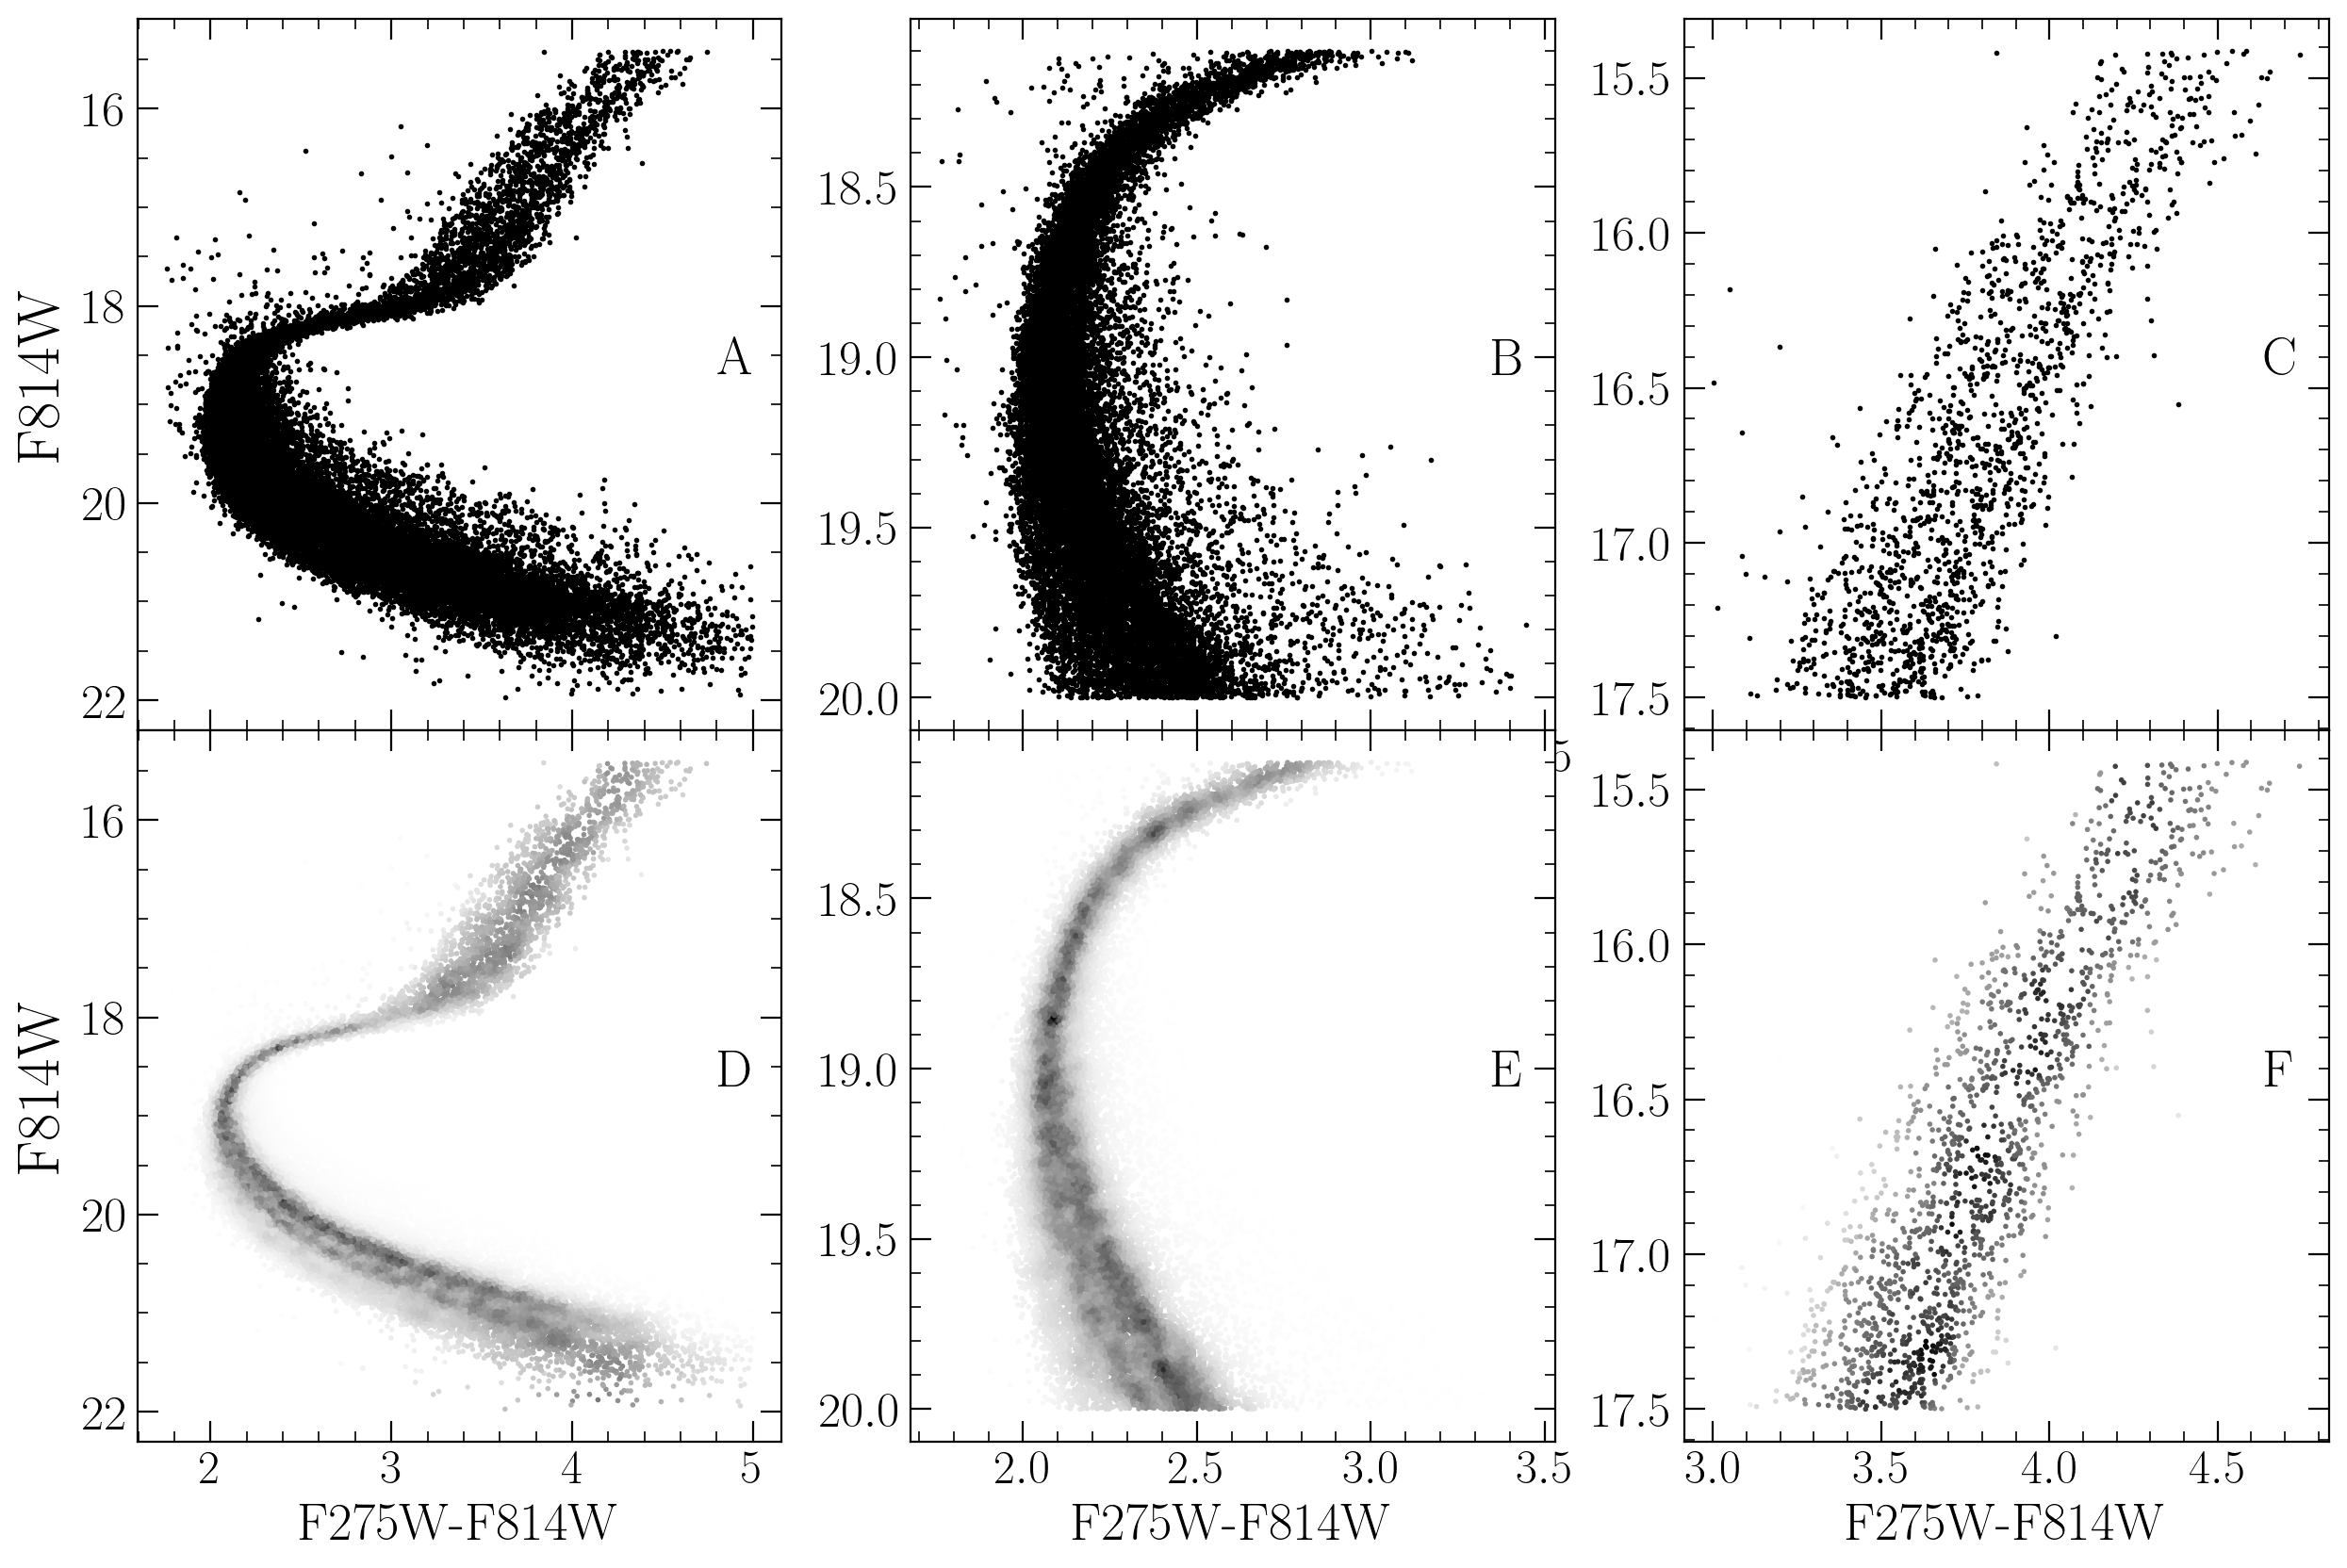
\includegraphics[width=0.9\textwidth]{src/figures/notebookFigures/DensityMapDemo.png}
	\label{fig:densityMapDemo}
	\caption{Density map demo showing density estimate over different parts of
	the evolutionary sequence. The left panel shows the density map over the
	entire evolutionary sequence, while the middle panel shows the density map
	over the main sequence and the right most panel shows the density map over
	the RGB. Figures in the top row are the raw CMD, while figures in the
	bottom row are colored by the density map.}
\end{figure*}

\fidanka can now exploit this density map to fit a better fiducial line to the
data, as the density map is far more robust to outliers. There are multiple
algorithms we implement to fit the fiducial line to the color-density profile
in each magnitude bin (Figure \ref{fig:densityBinsDemo}); they are explained in more detail in the \fidanka
documentation. However, of most relevance here is the Bayesian Gaussian Mixture
Modeling (BGMM) method. BGMM is a clustering algorithm which, for some fixed
number of n-dimensional Gaussian distributions, $K$, determines the mean, covariance, and
mixing probability (somewhat analogous to amplitude) of each $k^{th}$
distribution, such that the local lower bound of the evidence of each star
belonging strongly to a single distribution is maximized. 

\begin{figure}
	\centering
	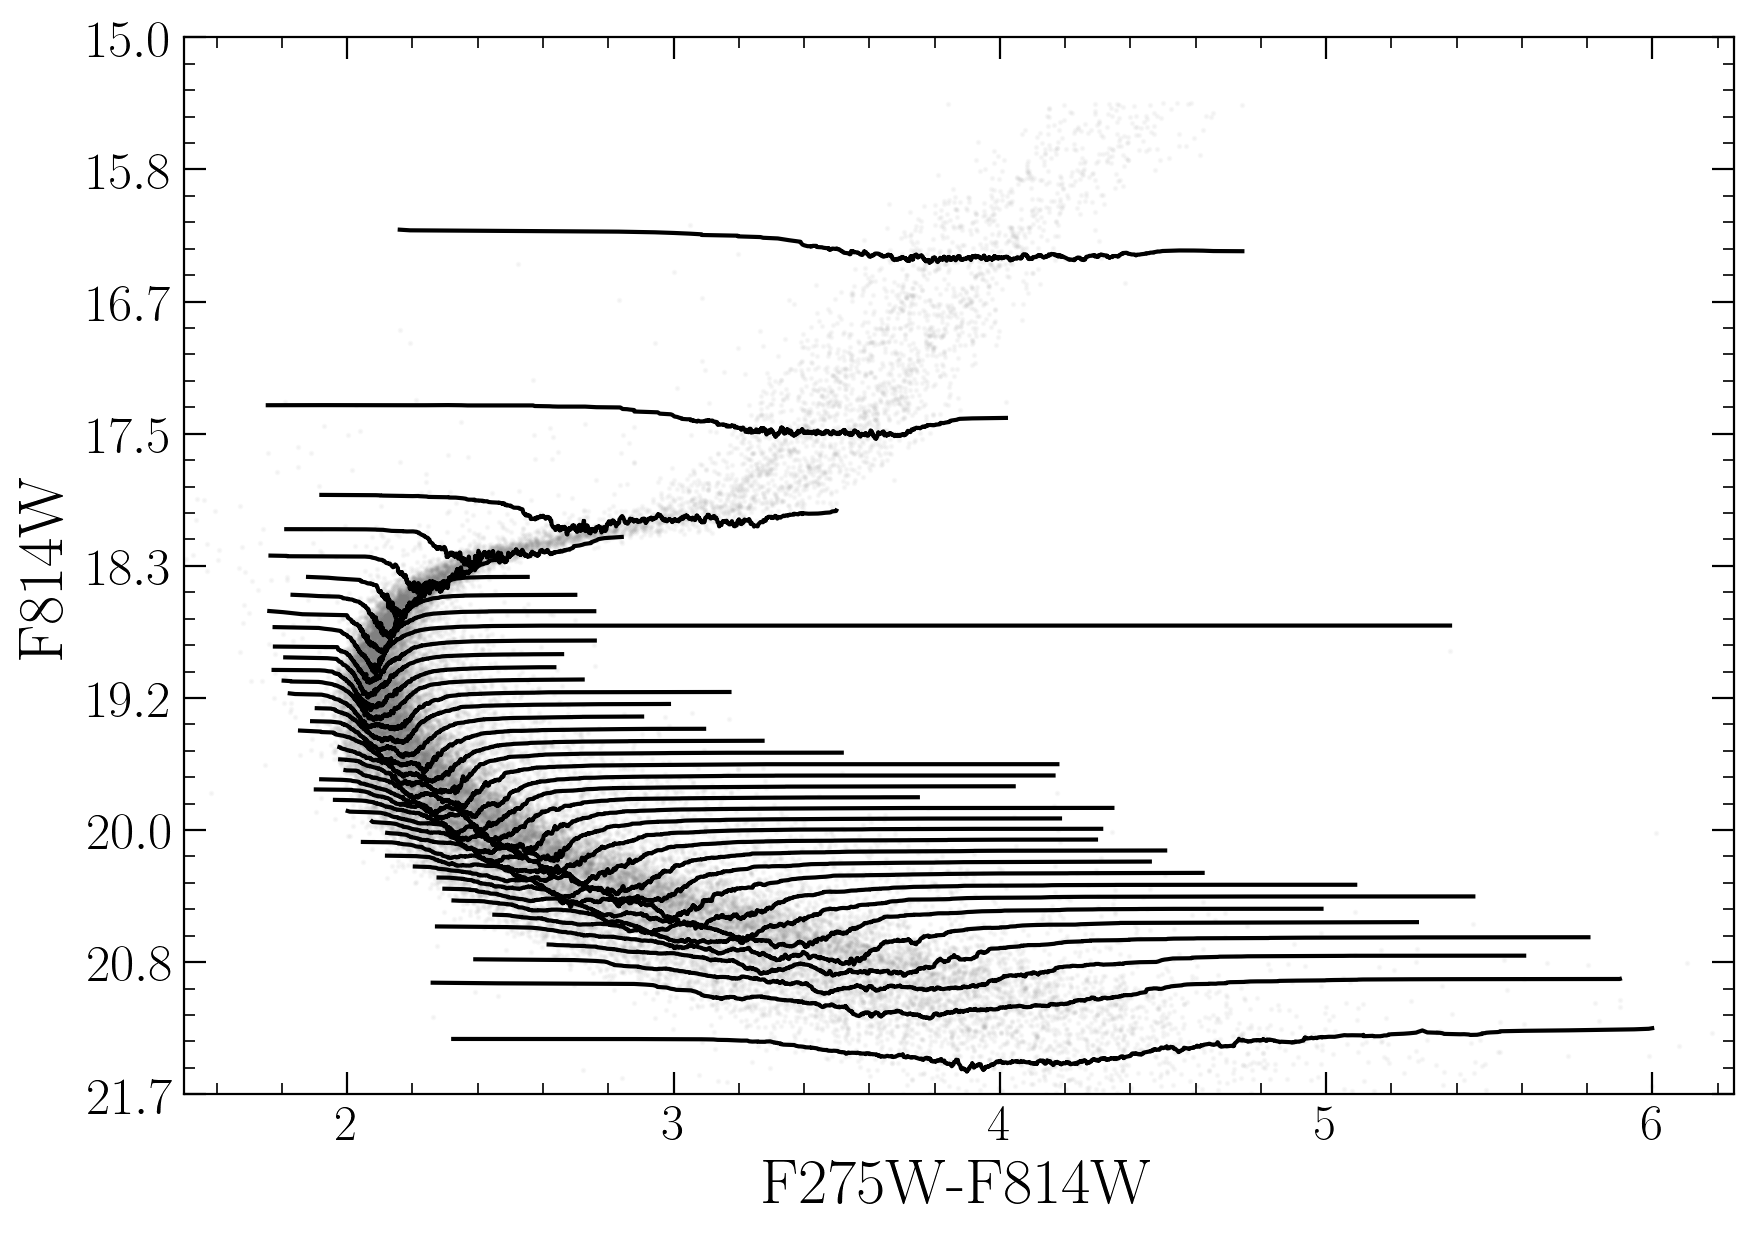
\includegraphics[width=0.45\textwidth]{src/figures/notebookFigures/DensityBinsDemo.png}
	\label{fig:densityBinsDemo}
	\caption{CMD where points are colored by density. Lines show the
	density-color profile in each magnitude bin. In this figure adaptive
	binning targeted 1000 stars per bin}
\end{figure}

Maximization is preformed using the Dirichlet process, which is a
non-parametric Bayesian method of determining the number of Gaussian distributions, $K$,
which best fit the data \citep{Ferguson1973, scikit-learn}. Use of the Dirichlet process
allows for dynamic variation in the number of inferred populations from
magnitude bin to magnitude bin. Specifically, populations are clearly visually
separated from the lower main sequence through the turn off; however, at the
turn off and throughout much of the subgiant branch, the two visible
populations overlap due to their extremely similar ages \citep[i.e.][]{Jordan2002}. The Dirichlet process allows for the BGMM method to infer a single
population in these regions, while inferring two populations in regions where
they are clearly separated. More generally, the use of the Dirichlet process
removes the need for a prior on the exact number of populations to fit. Rather,
the user specifies a upper bound on the number of populations within the
cluster. An example bin (F814W = 20.6) is shown in Figure \ref{fig:BGMMDist}.

\begin{figure*}
	\centering
	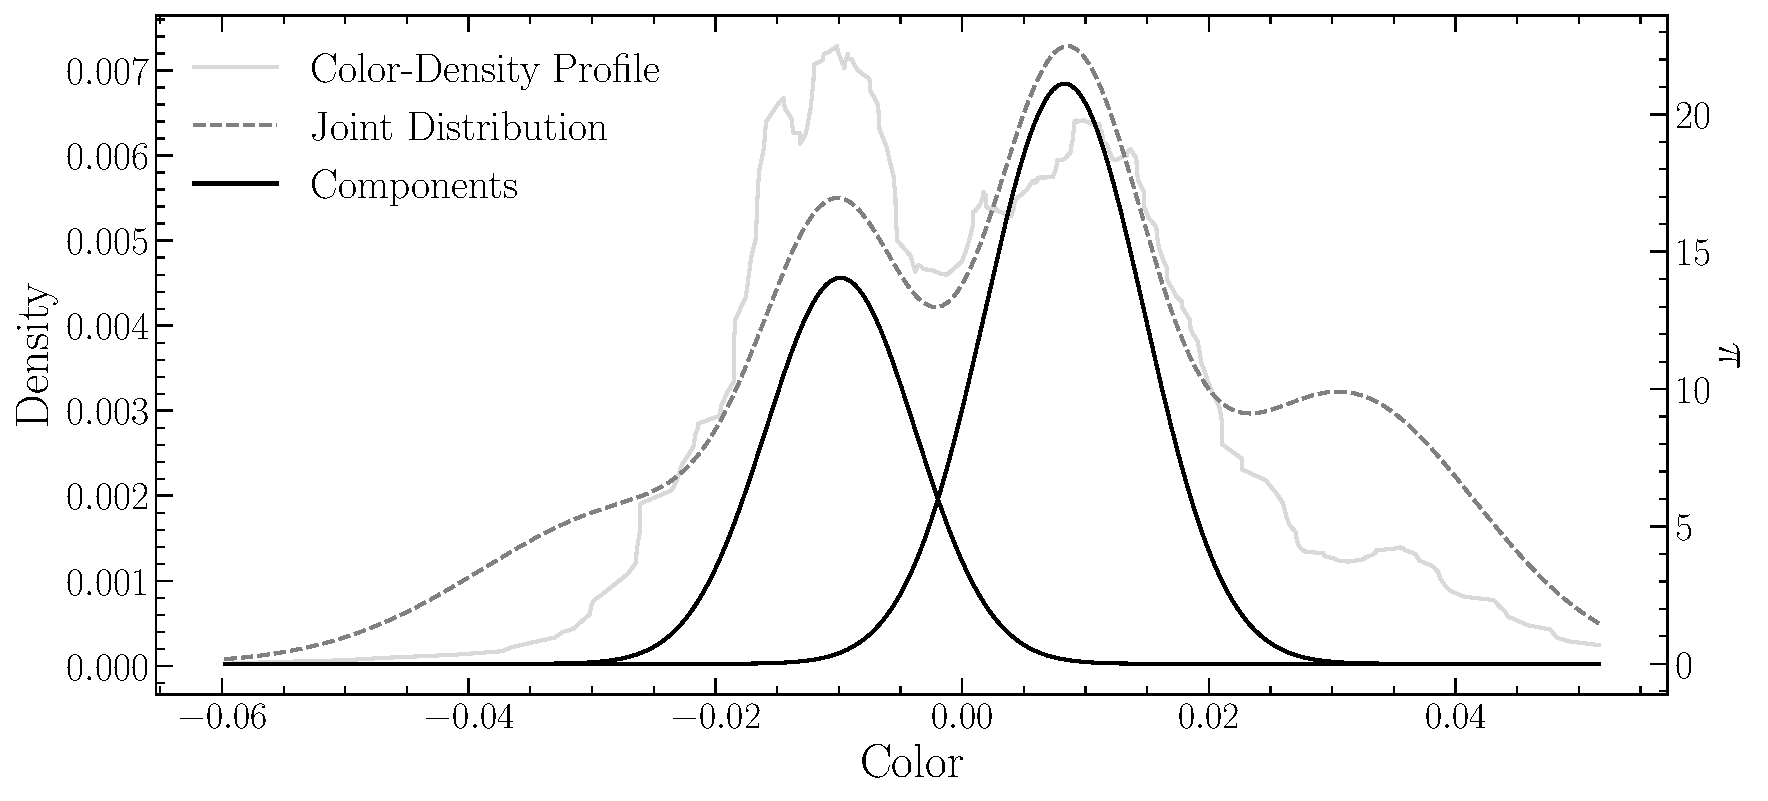
\includegraphics[width=0.9\textwidth]{Notebooks/Figures/BGMMMixingBin.pdf}
	\caption{Example of BGMM fit to a magnitude bin. The grey line shows the
	underlying color-density profile, while the black dashed-line shows the
	joint distribution of each BGMM component. The solid black lines show the
	two selected components.}
	\label{fig:BGMMDist}
\end{figure*}

\fidanka's BGMM method first breaks down the verticalized CMD into magnitude
bins with uniform numbers of stars per bin (here we adopt 250). Any stars left
over are placed into the final bin. For each bin a BGMM model with a maximum of
5 populations is fit to the color density profile. The number of populations is
then inferred from the weighting parameter (the mixing probability) of each
population. If the weighting parameter of any $k^{th}$ components less than
{\color{blue}0.05}, then that component is considered to be spurious and
removed. Additionally, if the number of populations in the bin above and the
bin below are the same, then the number of populations in the current bin is
forced to be the same as the number of populations in the bin above. Finally,
the initial guess fiducial line is added back to the BGMM inferred line. Figure
\ref{fig:vertFit} shows the resulting fiducial line(s) in each magnitude bin
for both a verticalized CMD and a non verticalized CMD.

\begin{figure}
	\centering
	\includegraphics[width=0.45\textwidth]{Notebooks/Figures/vertFit.png}
	\caption{CMD where points are colored by density. Line trace the infered 
	fiducial line(s) in each magnitude bin.}
	\label{fig:vertFit}
\end{figure}

This method of fiducial line extraction effectively discriminated between
multiple populations long the main sequence and RGB of a cluster, while
simultaneously allowing for the presence of a single population along the MSTO
and subgiant branch. 

We can adapt this density map based BGMM method to consider photometric
uncertainties by adopting a simple Monte Carlo approach. Instead of measuring
the fiducial line(s) a single time, \fidanka can measure the fiducial line(s)
many times, resampling the data with replacement each time. For each resampling
\fidanka adds a random offset to each filter based on the photometric
uncertainties of each star. From these $n$ measurments the mean fiducial line
for each sequence can be identified along with upper and lower bound confidence
intervals in each magnitude bin.

\subsection{Stellar Population Synthesis}
In addition to measuring fiducial lines, \fidanka also includes a stellar
population synthesise module. This module is used to generate synthetic CMDs
from a given set of isochrones. This is of primary importance for binary
population modelling. The module is also used to generate synthetic CMDs for
the purpose of testing the fiducial line extraction algorithms against priors.

\fidanka uses MIST formatted isochrones \citep{Dotter2016} as input along
with distance modulus, B-V color excess, binary mass fraction, and bolometric
corrections. An arbitrarily large number of isochrones may be used to define an
arbitrary number of populations. Synthetic stars are samples from each
isochrone based on a definable probability (for example it is believed that
$\sim90\%$ of stars in globular clusters are younger population
{\color{red}[CITATION]}). Based on the metallicity, $\mu$, and E(B-V) of each
isochrone, bolometric corrections are taken from bolometric correction tables.
Where bolometric correction tables do not include exact metallicities or
extinctions a linear interpolation is preformed between the two bounding
values. {\color{red}[FIGURE]} shows an example of a synthetic CMD generated
from a set of 2 NGC 2808 isochrones as well as a comparison between those
isochrones and the measured fiducial line of the synthetic population.

\subsection{Isochrone Optimization}
The optimization routines in \fidanka will find the best fit distance modulus,
B-V color excess, and binary number fraction for a given set of isochrones. If
a single isochrone is provided then the optimization is done by minimizing the
$\chi^2$ of the perpendicular distances between an isochrone and a fiducial
line. If multiple isochrones are provided then those isochrones are first used
to run stellar population synthesis and generate a synthetic CMD. The
optimization is then done by minimizing the $\chi^2$ of both the perpendicular
distances between and widths of the observed fiducial line and the fiducial
line of the synthetic CMD.


\subsection{Fidanka Testing}
In order to validate fidanka we have run an series of injection recovery tests
using \fidanka's population synthesis routines to build various synthetic
populations and \fidanka's fiducial measurement routines to recover these
populations. Each population was generated using the initial mass function
given in \citep{Milone2012} for the redmost population ($\alpha=-1.2$).
Further, every population was given a binary population fraction of 10\%,
distance uniformly sampled between 5000pc and 15000pc, and a B-V color excess
uniformly sampled between 0 and 0.1. Finally, each synthetic population was
generated using a fixed age  uniformlly sampled between 7 Gyr and 14 Gyr. An
example synthetic population along with its associated best fit isochrone are
shown in Figure \ref{fig:ValidationBestFit}.

\begin{figure}
  \centering
  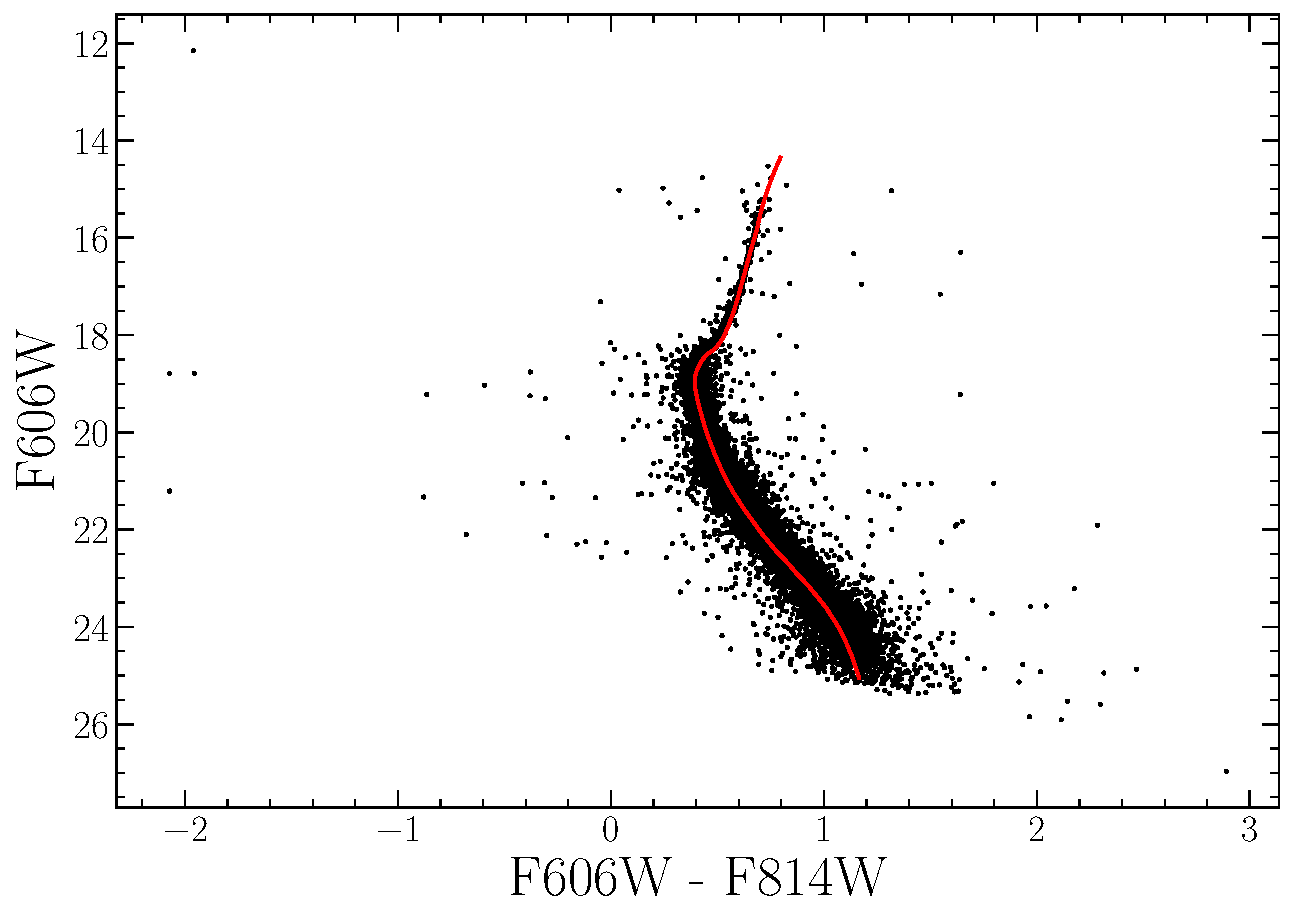
\includegraphics[width=0.45\textwidth]{src/figures/ExtractedIsoFit.pdf}
  \caption{Synthetic population generated by fidanka at 10000pc with E(B-V) = 0, and an age of 12 Gyr along with the best fitting isochrone. The best fit paremeters are derived to be $mu=15.13$, E(B-V)=0.001, and an age of 12.33 Gyr.}
  \label{fig:ValidationBestFit}
\end{figure}

For each trial we use \fidanka to measure the fiducial line and then optimize that fiducial line against the originating isochrone to esimate distance modulus, age, and color B-V excess. Figure \ref{fig:validationDist} is built from 1000 runs of these trials and show the mean and width of the percent error distributions for $\mu$, $E(B-V)$, and age. In general \fidanka is able to recover distance modulii effectively with age and E(B-V) reovery falling in line with other literature that does not cosider the CMD outside of the main sequence, main sequence turn off, sub giant, and red giant branches; specifically, it should be noted that \fidanka is not setup to model the horizontal branch.

\begin{figure}
  \centering
  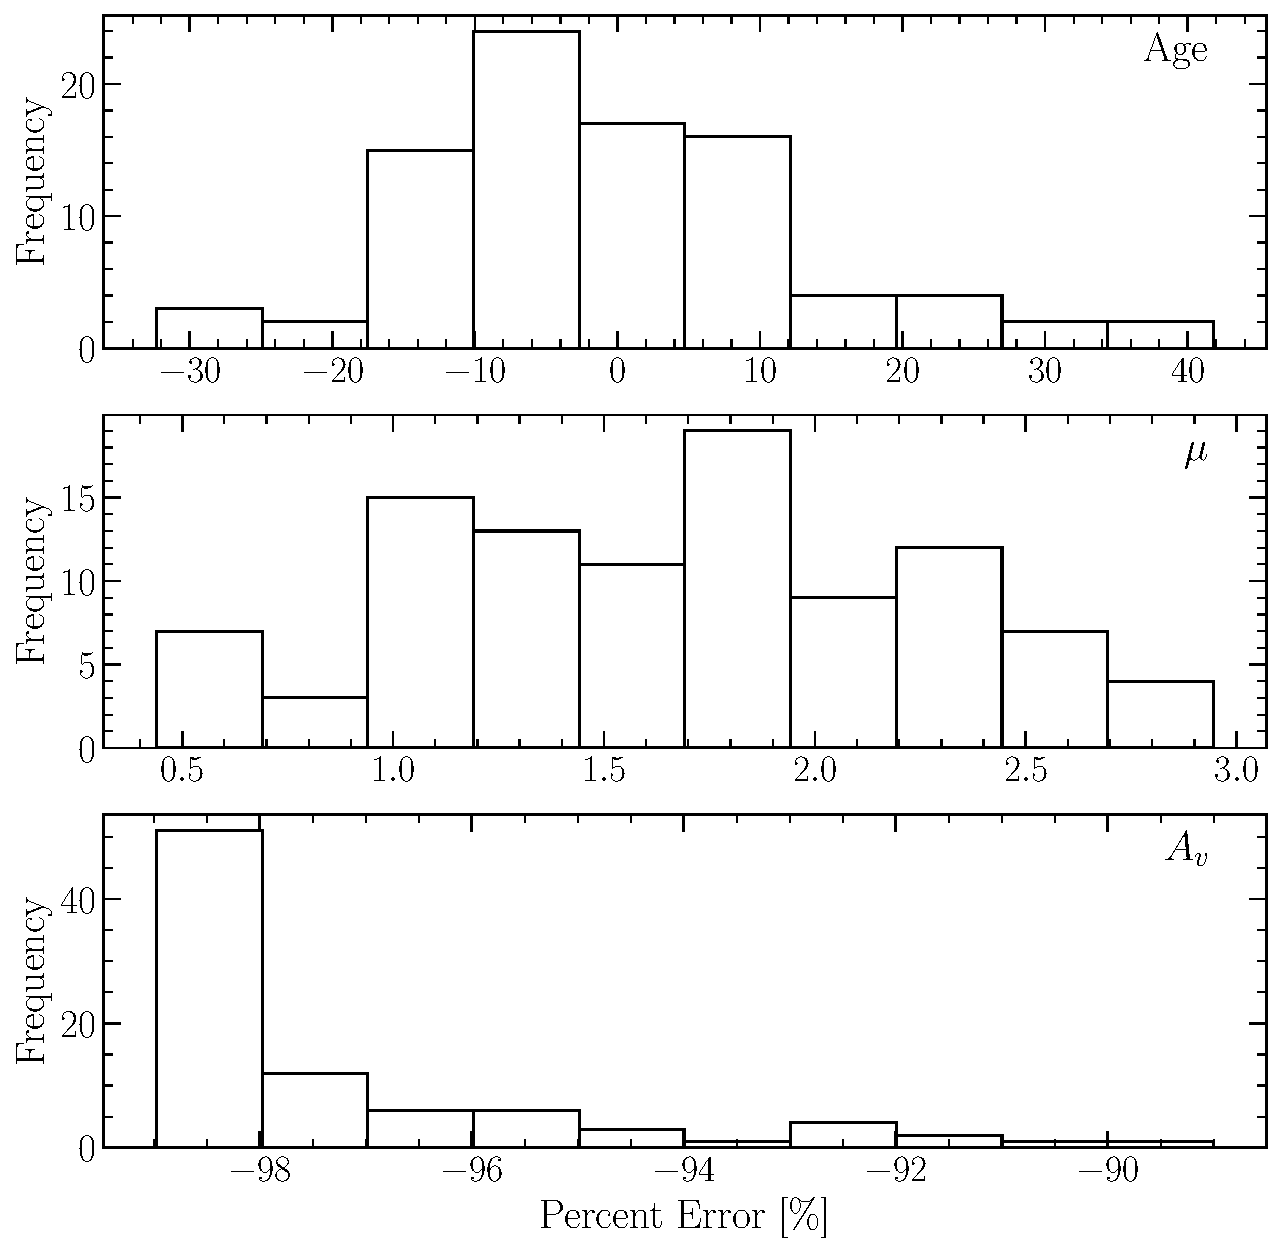
\includegraphics[width=0.45\textwidth]{src/figures/DistributionOfErrors.pdf}
  \caption{Percent Error distribution for each of the three deriver parameters. Note that these values will be sensitive to the magnitude uncertainties of the photometry. Here we made use of the ACS artificial star tests to estimate the uncertanties. {\color{blue}Note that currently this is built with 100 runs, these take a long time so currently re running with 1000 runs.}}
  \label{fig:validationDist}
\end{figure}


\section{Isochrone Fitting}\label{sec:isoFit}
We fit pairs of isochrones to the HUGS data for NGC 2808 using \fidanka, as
descrbed in \S \ref{sec:fidanka}. Two isochrones, one for Population A and one
for Population E are fit simultaneously. These isochrones are constrained to
have distance modulus, $\mu$, and color excess, E(B-V) which agree to within
0.5\% and an ages which agree to within 1\%. Moreover, we constrain the mixing length, $\alpha_{ML}$, for any two
isochrones in a set to be within 0.5 of one and other. For every isochrone in
the set of combination of which fulfilling these constraints $\mu$, $E(B-V)$,
Age$_{A}$, and $Age_{B}$ are optimized to reduce the $\chi^{2}$ distance
($\chi^{2} = \sum\sqrt{\Delta \text{color}^{2} + \Delta \text{mag} ^{2}}$)
between the fiducial lines and the isochrones. Because we fit fiducial lines
directly, we do not need to consider the binary population fraction, $f_{bin}$,
as a free parameter.

The best fit isochrones are shown in Figure \ref{fig:BestFitResults} and
optimized parameters for these are presented in Table \ref{tab:BestFitResults}.
We find helium mass fractions that are consistent with those identified in past
literature \citep[e.g.][]{Milone2015}. Note that our helium mass fraction grid
has a spacing of 0.03 between grid points and we are therefore unable to
resolve between certain proposed helium mass fractions for the younger sequence
(for example between 0.37 and 0.39).

\begin{figure*}
  \centering
  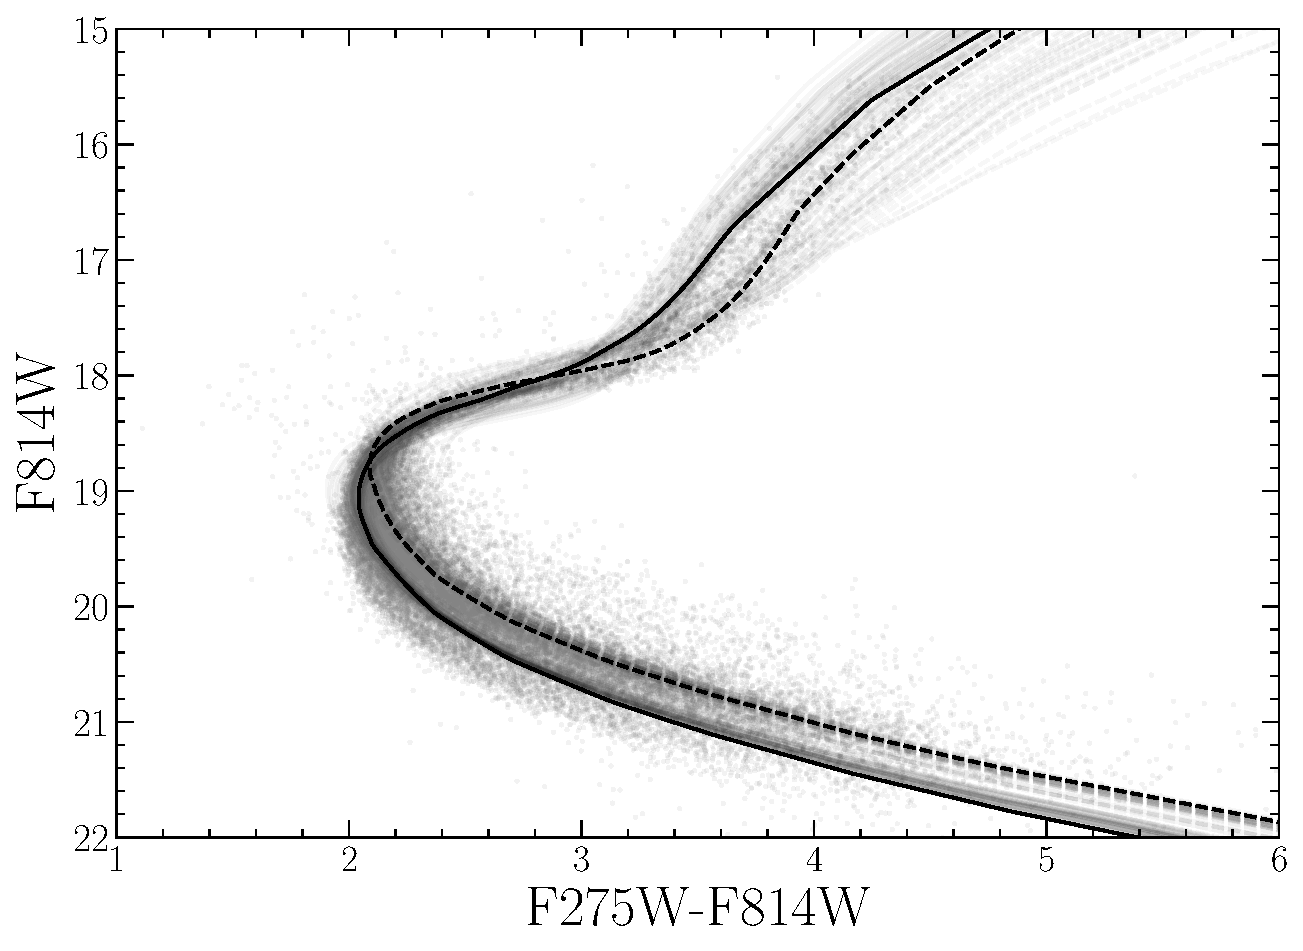
\includegraphics[width=0.9\textwidth]{src/figures/BestFitResults.pdf}
  \caption{Best fit isochrone results for NGC 2808. The best fit population A
  and E models are shown as black lines. The following 50 best fit models are
  presented as grey lines. The solid black line is fit to population A, while
  the dashed black line is fit to population E.}
  \label{fig:BestFitResults}
\end{figure*}

\begin{table*}
  \centering
  \begin{tabular}{c | c c c c c c}
    \hline
    Population & Age & Distance Modulus & Extinction & Y & $\alpha_{ML}$ & $\chi^{2}_{\nu}$\\
    & [Gyr] & & [mag] & & &\\
    \hline
    \hline
    A & 12.996$^{+0.87}_{-0.64}$ & 15.021 & 0.54 & 0.24 & 2.050 & 0.021\\
    E & 13.061$^{+0.86}_{-0.69}$ & 15.007 & 0.537 & 0.39 & 1.600 & 0.033 \\
    \hline
  \end{tabular}
  \caption{Best fit parameters derived from fitting isochrones to the fiducual lines derived from the NCG 2808 photometry. The one sigma uncertainty reported on population age were determined from the 16th and 84th percentiles of the distribution of best fit isochrones ages.}
  \label{tab:BestFitResults}
\end{table*}


Past literature \citep[e.g. ][]{Milone2015, Milone2018} have found helium mass
fraction variation from the low redmost to bluemost populations of $\sim 0.12$.
Here we find a helium mass fraction variation of 0.15 which, given the spacing
of the helium grid we use \textbf{is consistent with these past results}.

\subsection{The Number of Populartions in NGC 2808}
In order to estimate the number of populations which ideally fit the NGC 2808
F275W-F814W photometry without overfitting the data we make use of silhouette
analysis \citep[][and in a similar manner to how \citet{Valle2022} preform
their analysis of spectroscopic data]{ROUSSEEUW198753}. We find the average
silhouette score for all tagged clusters identified using BGMM in all magnitude
bins over the CMD using the standar python module \texttt{sklearn}. Figure
\ref{fig:clusterAn} shows the silhouette analysis results and that two
populations fit the photometry most ideally. This is in line with what our BGMM
model predicts for the majority of the the CMD.

{\bf While we make use a purley CMD based approach in this work, other
literature has made use of Chromosome Maps. These consist of implicitly
verticalized pseudo colors. In the chromosome map for NGC 2808 there may be
evidence for more than two populations; however, the process of transforming
magnitude measurements into chromosome space results in dramatically increased
uncertanties for each star. We find a mean fractional uncertantie for
chromosome parameters of $\approx1$ when starting with magnutude
measurements having a mean best-case (i.e. uncertainty assumed to only be due
to Poisson statistics) fractional uncertainty of $\approx 0.0005$. Because of
how \fidanka operates, i.e. resampling a probabilty distribution for each star
in order to idenfify clusters, we are unable to make statisitcally meaningful
statements from the chromosome map}

\begin{figure}
  \centering
  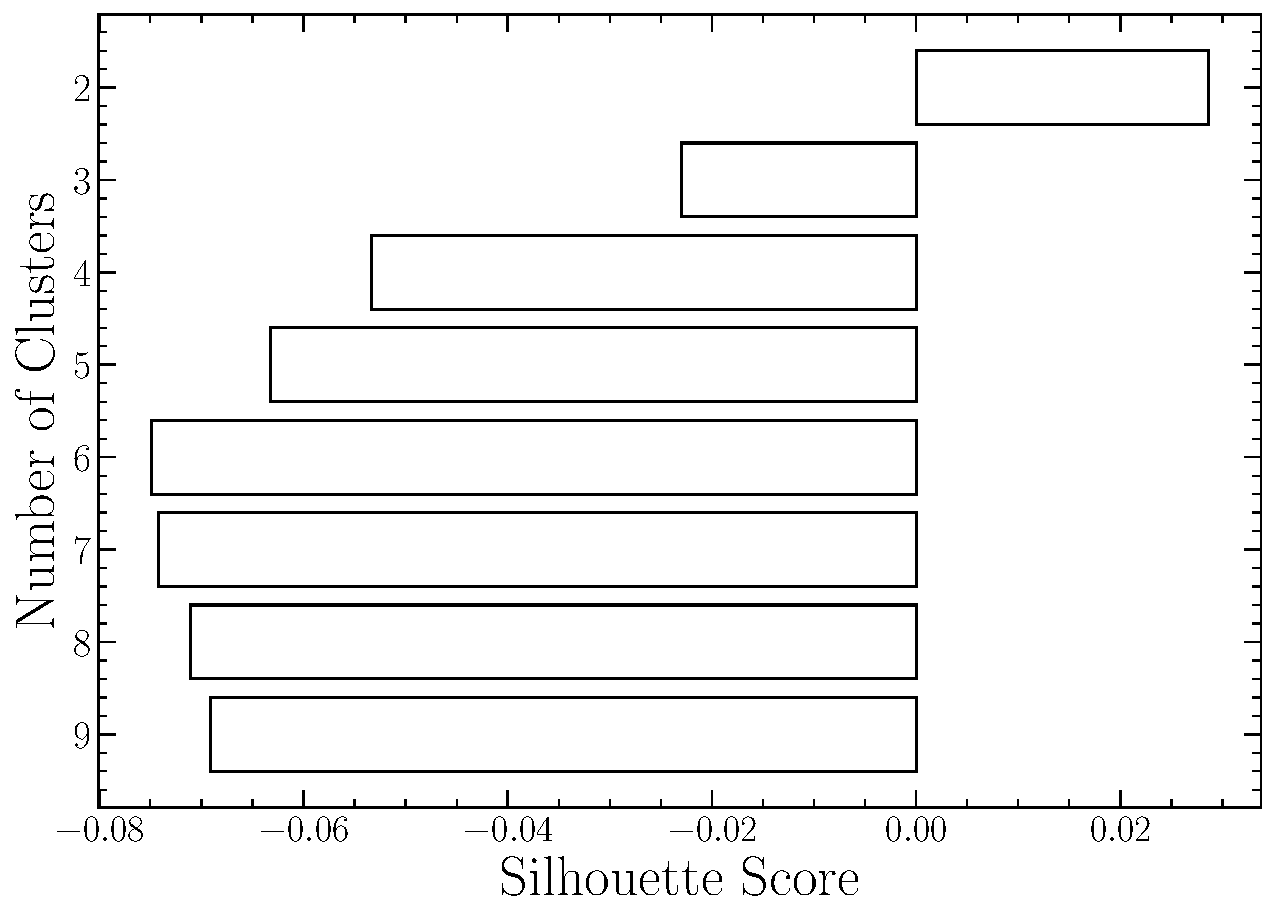
\includegraphics[width=0.45\textwidth]{src/figures/ClusterAnalysis.pdf}
  \caption{Silhouette analysis for NGC 2808 F275W-F814W photometry. The Silhouette scores
  are an average of score for each magnitude bin. Positive scores incidate that the clustering
  algorithm produced well distinguised clusters while negative scores indicate clusters which are not
  well distinguised.}
  \label{fig:clusterAn}
\end{figure}


\subsection{ACS-HUGS Photometric Zero Point Offset}
The Hubble legacy archive photometry used in this work is calibrated to the
Vega magnitude system. However, we have found that the photometry has a
systematic offset of $\sim0.026$ magnitudes in the F814W band when
compared to the same stars in the ACS survey (Figure \ref{fig:offset}). The
exact cause of this offset is unknown, but it is likely due to a difference in
the photometric zero point between the two surveys. A full correction of this
offset would require a careful re-reduction of the HUGS photometry, which is
beyond the scope of this work. We instead recognize a 0.02 inherent uncertainty
in the inferred magnitude of any fit when comparing to the ACS survey. This
uncertainty is small when compared to the uncertainty in the
distance modulus and should not affect the conclusion of this
paper. 

\begin{figure*}
  \centering
  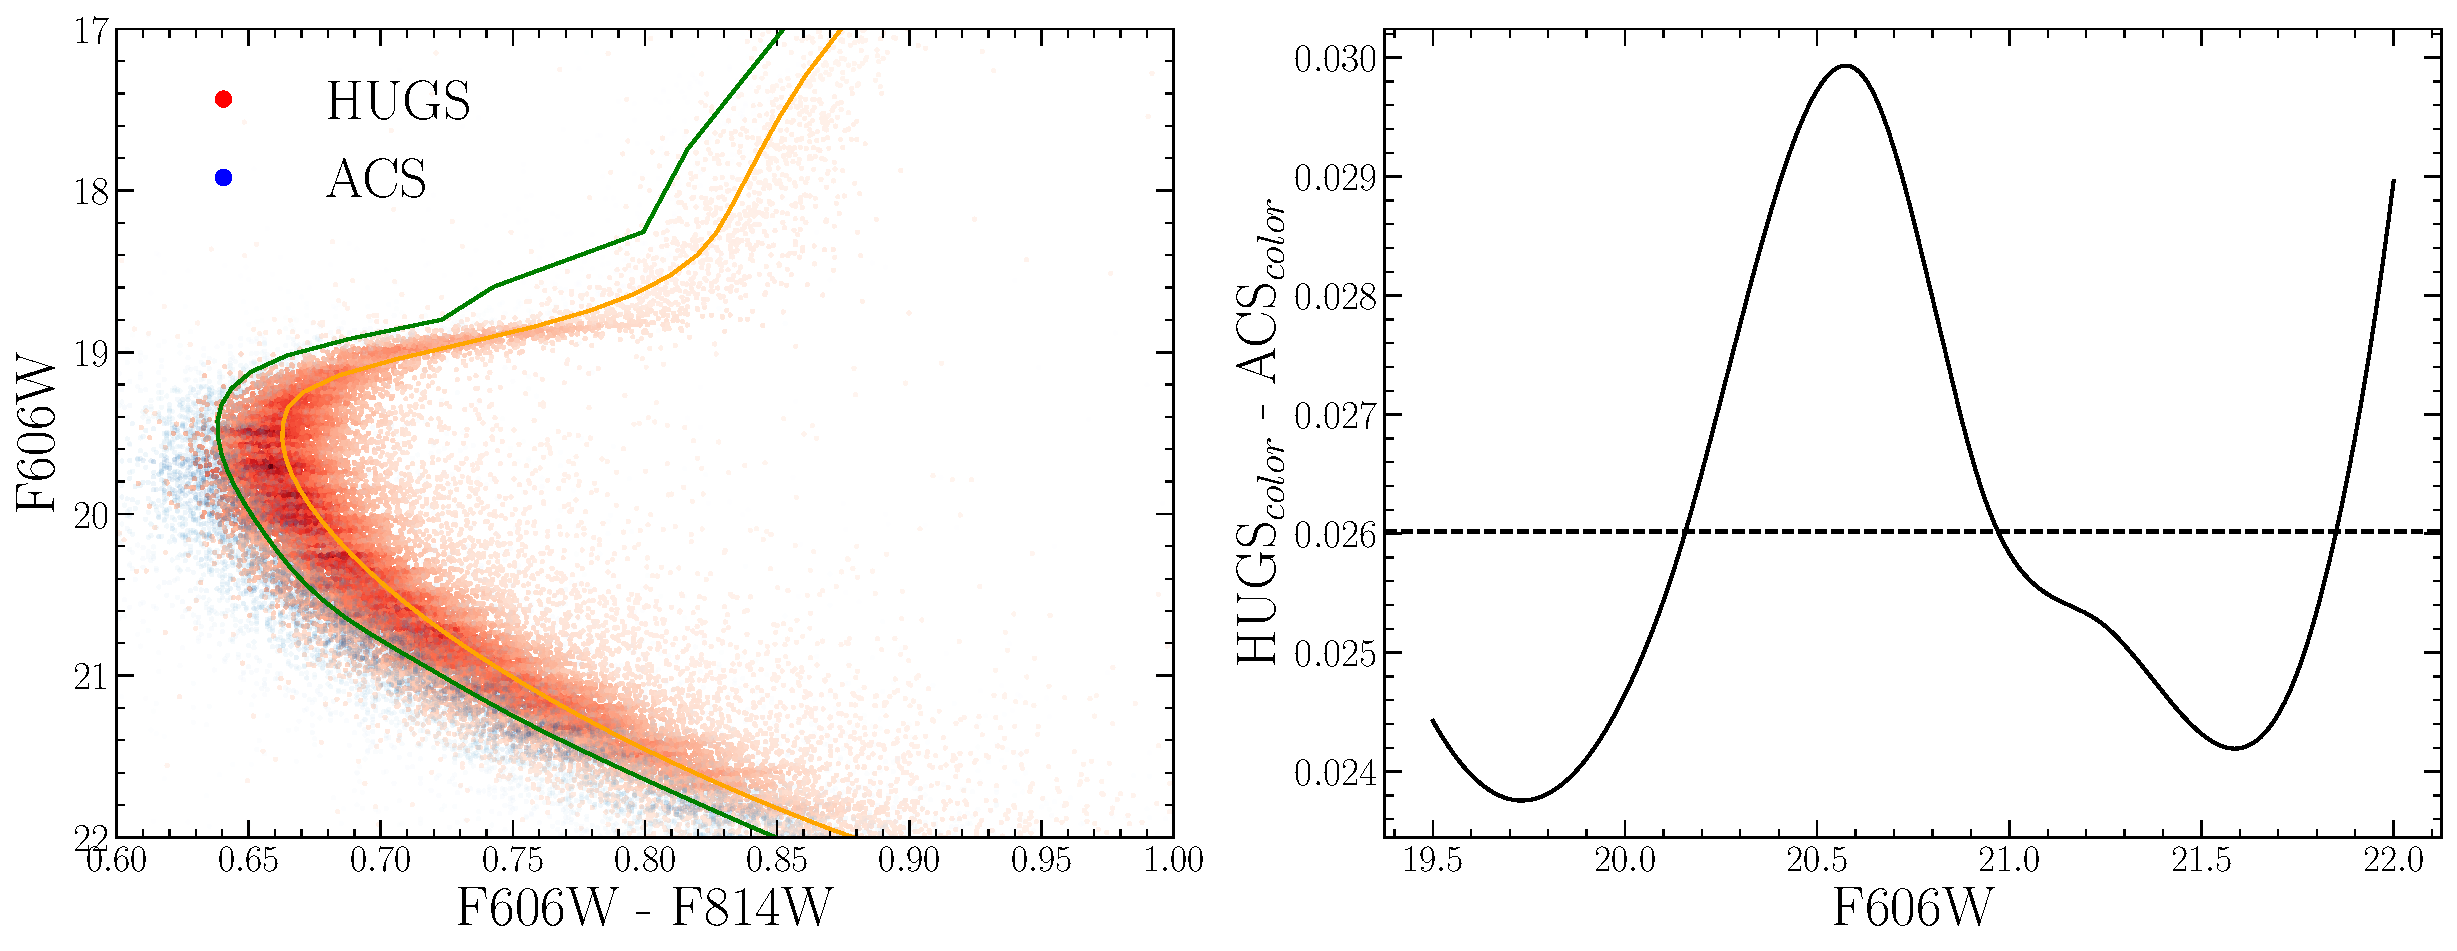
\includegraphics[width=0.90\textwidth]{src/figures/photometricOffset.pdf}
  \caption{(left) CMD showing the photometric offset between the ACS and HUGS data for NGC 2808. CMDs have been randomly subsampled and colored by point density for clarity. (right) Mean difference between the color of the HUGS and ACS fiducual lines at the same magnitude. Note that the ACS data is systematically bluer than the HUGS data.}
  \label{fig:offset}
\end{figure*}

The oberved photometric offset between ACS and HUGS reductions introduces a
systematic uncertainity when comparing parameters derived from isochrone fits
to ACS data vs those fit to HUGS data. Specifically, this offset introduces a
$\sim 2 Gyr$ uncertainity when comparing ages between ACS and HUGS. Moreover,
for two isochrone of the same age, only seperated by helium mass fraction, a
shift of the main sequence turn off of is also expected. Figure \ref{fig:HeMO}
shows this shift. Note a change in the helium mass fraction of a model by 0.03
results in an approximate 0.08 magnitude shift to the main sequence turn off
location. This means that the mean 0.026 magnitude offset we find in between
ACS and HUGS data corresponds to an additional approaximate 0.01 uncertainity
in the derived helium mass fraction when comparing between these two datasets. 

\begin{figure}
  \centering
  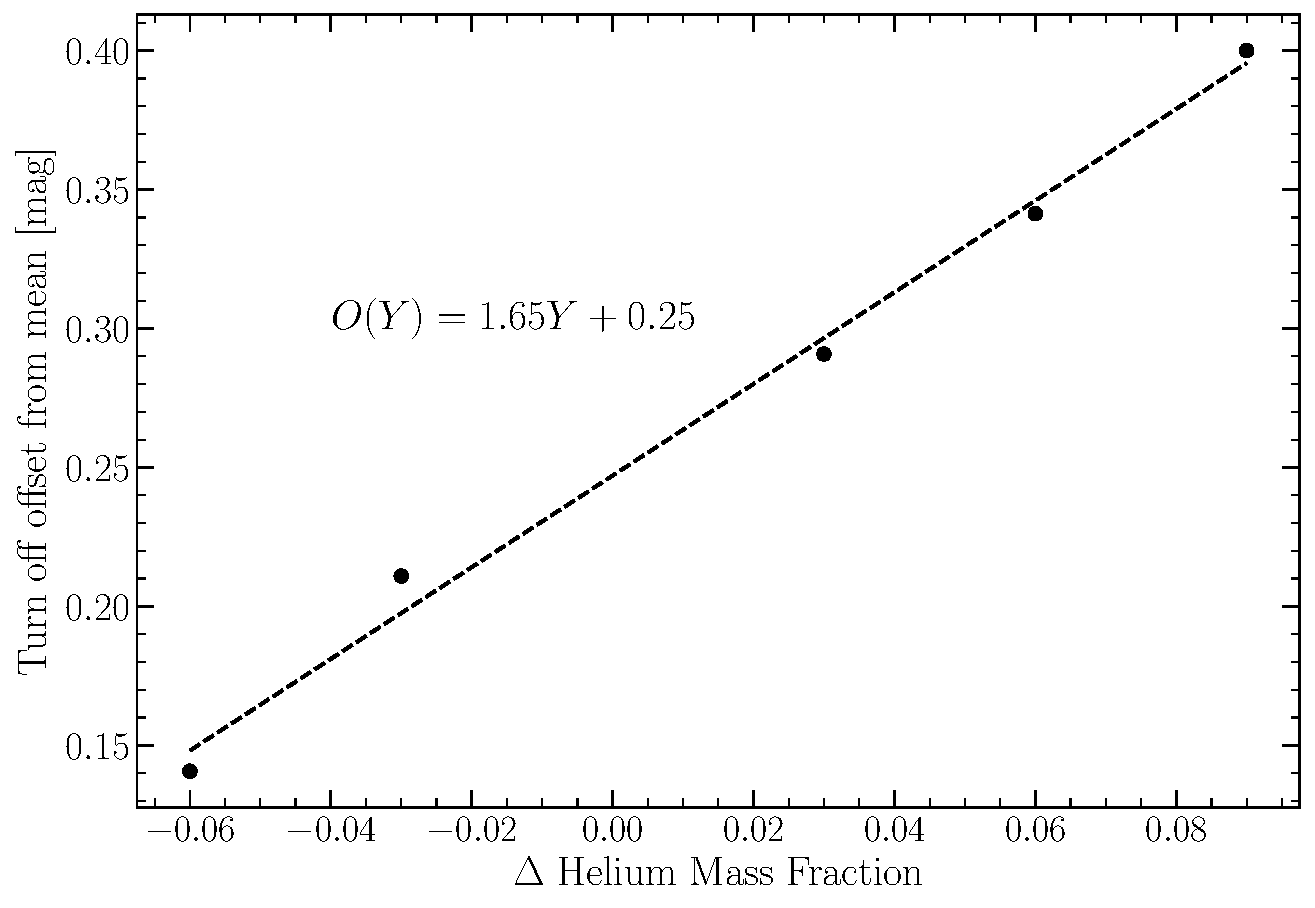
\includegraphics[width=0.45\textwidth]{src/figures/HeliumMeanOffset.pdf}
  \caption{Main sequence turn off magnitude offset from a guage helium mass fraction (Y=0.30 chosen). All main sequence turn off locations are measured at 12.3 Gyr {\color{blue} Should I make these contour surfaces for various ages?}}
  \label{fig:HeMO}
\end{figure}


\section{Results}\label{sec:results}
Using \fidanka we fit pairs of Population A + E isochrones to the HUGS data for
NGC 2808. Each pair of isochrones is allowed to vary in distance modulus,
reddening, relative helium mass fraction (A/E), and age. Any population pairs which vary by more than 1\% in distance modulus or B-V color excess are rejected. The $\chi^{2}$
distribution for the isochrone pairs is shown in Figure {\color{red}[FIGURE]}.
The best fit isochrones are shown in Figure \ref{fig:BestFitResults} and optimized
parameters for these are presented in Table {\color{red}[TABLE]}.

{\color{red} Need to make the chi2 dist plot still. Have all these values but need to figure out best way to visualize it}

\begin{figure}
  \centering
  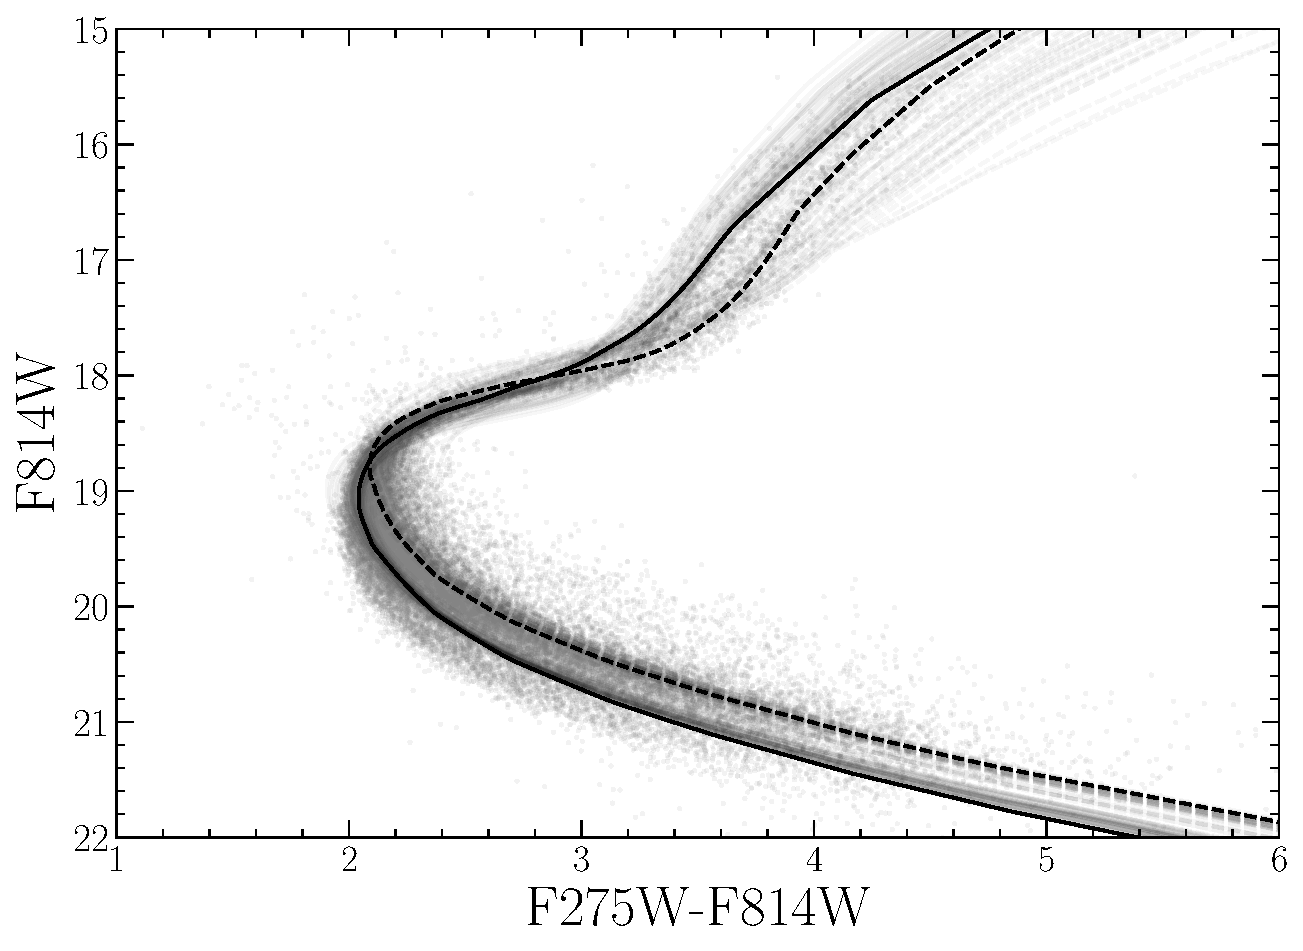
\includegraphics[width=0.45\textwidth]{src/figures/BestFitResults.pdf}
  \label{fig:BestFitResults}
  \caption{Best fit isochrone results for NGC 2808.}
\end{figure}

\begin{table*}
  \centering
  \begin{tabular}{c | c c c c c c}
    \hline
    population & age & distance modulus & extinction & Y & $\alpha_{ML}$ & $\chi^{2}_{\nu}$\\
    & [Gyr] & & mag & & &\\
    \hline
    \hline
    A & 12.3 & 14.91 & 0.54 & 0.24 & 1.901 & 0.014\\
    E & 14.3 & 14.96 & 0.54 & 0.39 & 1.750 & 0.017 \\
    \hline
  \end{tabular}
  \label{tab:BestFitResults}
  \caption{Best fit parameters derived from fitting isochrones to the fiducual lines derived from the NCG 2808 photometry.}
\end{table*}

{\color{blue} Currently are still seeing a discontinutiy in the isochrobne below the MSTO. This must be addressed before submission.}

\subsection{The Number of Populartions in NGC 2808}
\fidanka provides a somewhat straigtforward way to estimate the number of populations expected in a given magnitude bin given the observations. See Section \ref{sec:fidanka} for specific implimentaiton details. Here we preform an analysis of the number of populations seen in the NGC 2808 F814W-F274W vs F814W color-magnitude diagram. We find that for the majority of the main sequence and red giant branches BGMM prefers two populations; wherease, near the main sequnce turn off and on the majority of the subgiant branches BGMM prefers a single population model.

{\color{red}[FIGURE SHOWING BGMM population probability]}



% \input{src/sections/discussion.tex}

\section{Conclusion}\label{sec:conclusion}
{\color{red} Here we have preformed the first chemically self-consistnent
modeling of the Milky Way Globular Cluster NGC 2808. We find that, updated
atmospheric boundary conditions and opacity tables do not have a significant
effect on the inferred helium abundances of multiple populations.}



\begin{acknowledgments}
	This work has made use of the NASA astrophysical data system (ADS). We
	would like to thank Elisabeth Newton and Aaron Dotter for their support and
	for useful disscusion related to the topic of this paper. Additionally, we
	would like to thank Kara Fagerstrom, Aylin Garcia Soto, and Keighley
	Rockcliffe for their useful disscusion related to in this work. We
	acknowledge the support of a NASA grant (No. 80NSSC18K0634). 
\end{acknowledgments}

% \software{
% 	The Dartmouth Stellar Evolution Program (DSEP) \citep{Dotter2008},
% 	\texttt{FreeEOS} \citep{Irwin2012},
% 	\texttt{pyTOPSScrape} \citep{Boudreaux22}
% }


\bibliography{src/bib/ms}{}
\bibliographystyle{aasjournal}


\end{document}
